% =============================================================================
% CAPÍTULO 5 — volta 1, a última forma: a dependência que a margem não vê.
%
% O fracasso que o abre, com número na mão: dois mercados protegidos cada um no seu corte de
% 5% rompem juntos 7,17 vezes mais do que a independência prevê, e nenhum instrumento dos
% capítulos 2 e 4 pode ver isso — a informação não está em nenhuma das duas séries.
%
% A prova de cegueira é medida: deslocando só o pareamento do segundo mercado, a primeira
% perna rompe os MESMOS 315 dias e a razão contra a independência cai de 7,17 para 1,43.
%
% Medição: lab/experimentos/E05_dependencia.ipynb. Figuras: figuras/E05_dependencia_*.
% =============================================================================

\chapter{O dia em que tudo cai junto}
\label{cap:dependencia}

\section{O que a margem não vê}

Os três capítulos anteriores vigiaram uma série por vez: o corte, o vigia, a célula do
calendário. Todos eles leem uma margem, e este capítulo trata de duas ao mesmo tempo. Ele começa por uma
tentativa que qualquer mesa faz: proteger cada mercado no seu próprio corte de
\numPromessaPct\%, e supor que a proteção dos dois é a soma das duas.

O par é o índice americano e o brasileiro: \numDependenciaDias{} dias em que os dois têm
corte, dos \numPedacoDiasComuns{} em que os dois existiram, um quarto de século de mercado. Cada um rompeu o seu próprio corte na mesma taxa: \numDependenciaTaxaAPct\% dos dias de um
lado, \numDependenciaTaxaBPct\% do outro, ou \numDependenciaRompeA{} rompimentos e
\numDependenciaRompeB{} --- a promessa do primeiro capítulo sendo cumprida duas vezes.

Agora a conta que interessa: se os dois mercados fossem independentes, os dias em que os dois
rompem seriam o produto das duas taxas, e ao longo de \numDependenciaDias{} dias isso daria
\numDependenciaEsperadoDias{} dias. Aconteceram \numDependenciaJuntos: \numDependenciaJuntosPct\%
dos dias, contra os \numDependenciaEsperadoPct\% que a independência preveria. A razão entre o que se mediu e o que a independência previa é de \numDependenciaExcesso{} vezes.

Dito pela outra ponta, que é como quem carrega a posição sente: dos \numDependenciaRompeA{}
rompimentos do primeiro mercado, \numDependenciaAcompanhadosPct\% vieram acompanhados por um
rompimento do segundo. Somando as duas proteções, esperar-se-ia
\numDependenciaAcompanhadosIndependentePct\%. Essa fração é a dependência de cauda, e estimá-la de
uma amostra finita tem viés próprio \cite{garcin2026nonparametric}.

\section{A conta que a soma faz}

Vale escrever por que a soma erra, porque o erro não é de aritmética. Se as duas pernas fossem
independentes, a chance de as duas romperem no mesmo dia seria o produto das duas: é o que faz
a soma das proteções ser, ao mesmo tempo, correta e inútil. O produto supõe que saber de uma
perna não diga nada sobre a outra, e é exatamente isso que um dia ruim desmente.

\begin{proposicao}[o teto do par]\label{prop:teto-do-par}
Se cada perna rompe o próprio corte com probabilidade $p$, a chance de as duas romperem no mesmo
dia não passa de $p$, por mais forte que seja a dependência entre elas. A independência preveria
$p^{2}$, de modo que o par pode entregar até $1/p$ vezes o que a soma prevê.
\end{proposicao}

\begin{proof}
O acontecimento \emph{as duas rompem} está contido em \emph{a primeira rompe}, e a probabilidade
de um acontecimento não passa da probabilidade do que o contém: a chance conjunta não passa de
$p$. A independência é o outro extremo, com $p^{2}$, e a razão entre os dois extremos é $1/p$ ---
vinte no corte de \numPromessaPct\%.
\end{proof}

A medida que este capítulo usa não é a correlação, e a escolha é deliberada. Correlação é uma
média do miolo: ela resume os dias comuns, que são a maioria, e não tem motivo nenhum para
acertar na cauda, que é onde a conta é paga. O que se conta aqui é mais cru e mais direto:
quantos dias as duas romperam o próprio corte, contra quantos dias a independência preveria.
Nenhuma forma de dependência é suposta --- não há normalidade, não há cópula, não há parâmetro
---, só a contagem dos dias em que as duas séries existem.

A cota da \cref{prop:teto-do-par} diz quanto essa contagem pode andar: o par como veio entrega
\numDependenciaExcesso{} vezes o que a soma prevê, e o teto do corte de \numPromessaPct\% é de vinte
vezes.

\begin{figure}[htbp]
  \centering
  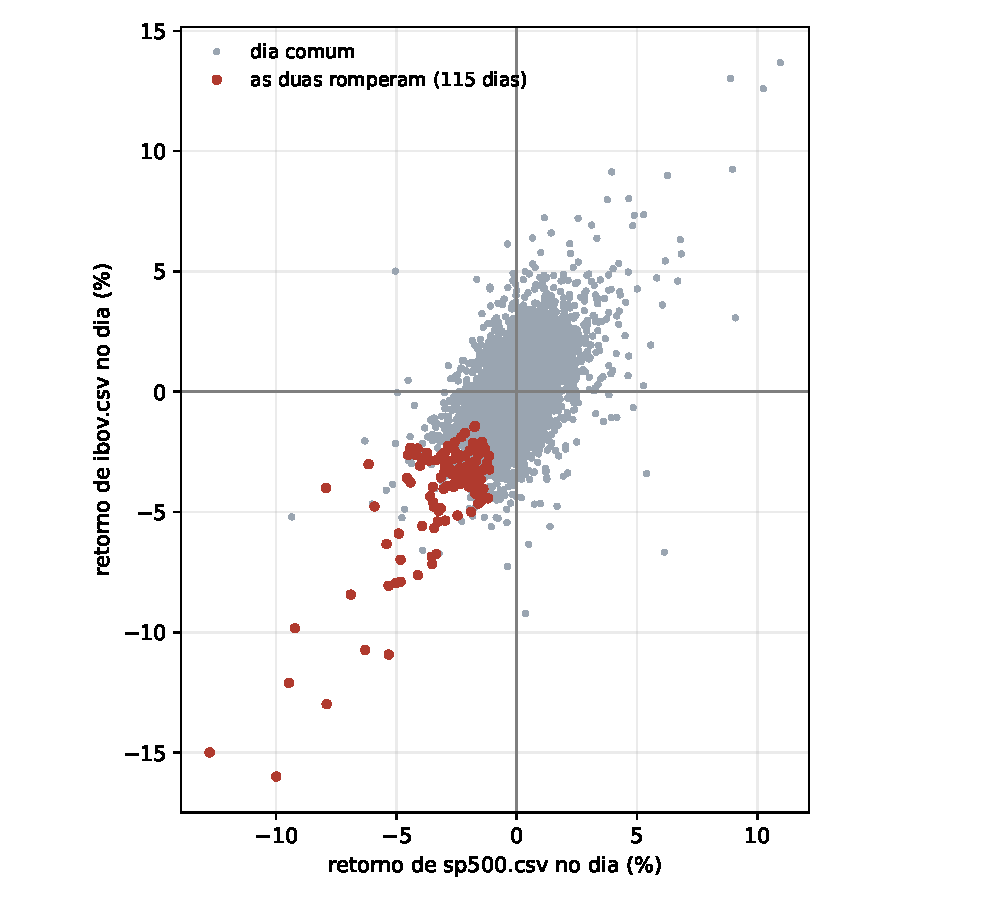
\includegraphics[width=0.82\linewidth]{figuras/E05_dependencia_1.pdf}
  \caption{Os dois mercados, dia a dia. Cada ponto é um dia, com o retorno de um no eixo
    horizontal e o do outro no vertical; as linhas em zero partem o plano em quadrantes. Os
    \numDependenciaJuntos{} dias em que as duas pernas romperam estão todos no quadrante de
    baixo à esquerda, e nenhum em qualquer outro lugar do plano.}
  \label{fig:nuvem}
\end{figure}

As duas retas do desenho marcam o zero de cada mercado, e o corte de cada dia fica bem mais fundo
que ele: o quadrante de baixo à esquerda é muito maior do que o punhado de pontos vermelhos que ele
contém. Quem passa o olho encontra ali todo dia de queda, e a figura marca outra coisa --- o dia em
que as duas pernas foram ao fundo juntas.

\section{O par é que decide}

Falta a parte difícil, que é mostrar que nada disso está em nenhuma das duas séries. A
experiência é simples e é decisiva: desloque o segundo mercado em um dia, em três semanas, em
um ano, em dois anos. Cada perna continua com os seus próprios números, na sua própria ordem;
o que muda é o \emph{par} --- qual dia de um mercado encontra qual dia do outro.

\begin{table}[htbp]
  \centering
  \begin{tabular}{lrr}
    \hline
    o par & rompe o primeiro & contra a independência \\
    \hline
    o que o mundo fez & \numDependenciaRompeA & \numDependenciaExcesso \\
    um dia depois & \numDependenciaRompeA & \numDependenciaAtrasoUmDiaExcesso \\
    três semanas depois & \numDependenciaRompeA & \numDependenciaAtrasoVinteEUmDiasExcesso \\
    um ano depois & \numDependenciaRompeA & \numDependenciaAtrasoUmAnoExcesso \\
    dois anos depois & \numDependenciaRompeA & \numDependenciaAtrasoDoisAnosExcesso \\
    \hline
  \end{tabular}
  \caption{A mesma série, com o par trocado. A coluna da esquerda é a que importa: a
    primeira perna rompe os mesmos \numDependenciaRompeA{} dias em todas as linhas, porque a
    série dela não foi tocada. O pareamento é a única coisa que mudou.}
  \label{tab:par}
\end{table}

A primeira coluna da tabela é a resposta inteira. A perna do primeiro mercado rompe os mesmos
\numDependenciaRompeA{} dias nas cinco linhas: a margem dela não se mexeu, e nenhum instrumento
que leia essa série --- nem a contagem do segundo capítulo, nem a célula do terceiro --- pode
distinguir uma linha da outra, porque não há nada a distinguir. O que muda é só a conta
conjunta, que cai de \numDependenciaExcesso{} vezes a independência para
\numDependenciaAtrasoUmDiaExcesso{} com um único dia de deslocamento, e para perto de um quando
o atraso passa de três semanas.

Um dia de deslocamento já destrói quase tudo, e isso diz onde a dependência mora: no mesmo dia.
A correlação conta a mesma história por outro caminho --- \numDependenciaCorrelacao{} com o par
real, \numDependenciaAtrasoUmDiaCorrelacao{} com o par deslocado por um dia ---, e é útil aqui
só como conferência, porque ela é a média que o miolo vê e não a contagem que a cauda paga.

\section{O controle}

Antes de aceitar um número desses, vale olhar o que ele dá quando não há nada para medir. Dois
mundos sorteados independentes, com a mesma rotina de corte: as razões
\numDependenciaExcesso{}, \numDependenciaAtrasoUmDiaExcesso{} e companhia não significam nada se
a conta também der sete quando as duas séries não têm nada a ver uma com a outra.

Sorteamos duas séries independentes do tamanho do par real e medimos o mesmo número: \numDependenciaControleExcesso{} vezes a independência. É o que tem de dar: a medida vale um
quando não há dependência, e é contra esse um que as outras linhas se leem.

\section{O que a proteção individual não cobre}

Falta o preço, e ele é o que decide se o número interessa a quem carrega a posição. Montamos a
carteira de peso igual nas duas pernas e olhamos a perda média em dois conjuntos de dias: os
\numDependenciaJuntos{} em que as duas romperam, e os quatrocentos e dois em que só uma rompeu.

No dia em que as duas rompem, a carteira perde \numDependenciaPerdaJuntosPct\%; no dia em que só
uma rompe, perde \numDependenciaPerdaUmaPernaPct\%. A razão entre as duas perdas é de \numDependenciaPerdaRazao{} vezes, e o dia conjunto é mais fundo que o dia de uma perna só: é justamente aquele em que as duas proteções são chamadas ao mesmo tempo.

\begin{figure}[htbp]
  \centering
  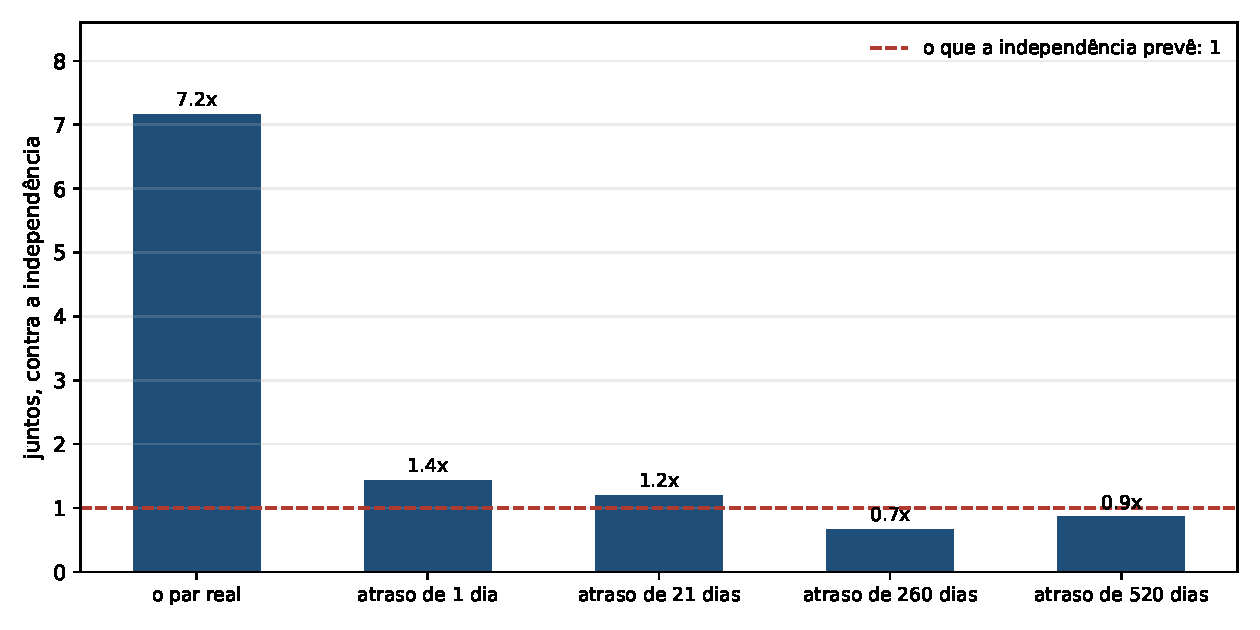
\includegraphics[width=\linewidth]{figuras/E05_dependencia_2.pdf}
  \caption{A barra da esquerda é o par como o mundo fez; as outras quatro são o mesmo par com o
    segundo mercado deslocado, e a linha tracejada é o que a independência prevê.
    Quase toda a dependência morre com um único dia de deslocamento.}
  \label{fig:par}
\end{figure}

\section{O que fica}

Fica um instrumento, e ele é pequeno o bastante para caber numa frase: \textbf{conte os dias em
que as duas coisas rompem, e compare com o que a independência preveria}. A razão entre os dois
não supõe forma nenhuma de dependência, não precisa de normalidade nem de cópula, e responde à
pergunta que a soma das proteções responde errado.

E fica o que este capítulo mostrou sobre os capítulos anteriores, que é mais desconfortável do
que o número. O vigia do segundo capítulo e a célula do terceiro leem margens, e o pareamento não mora em margem alguma. Mudar o par deixa as duas séries idênticas a si mesmas e muda a conta. Não é que aqueles instrumentos sejam fracos --- é que a pergunta que este capítulo faz não
é uma pergunta sobre uma série.

O fracasso seguinte nasce do próprio número que ficou. \numDependenciaExcesso{} vezes a
independência é uma média sobre um quarto de século de pregões; ela diz que os dois caem juntos mais do que a
sorte explicaria, e não diz \emph{desde quando}. Existe um dia em que a dependência mudou --- em
que o par deixou de valer o que valia ---, e a mesma estatística que responde "que conjunto ainda
vale" responde "em que instante ele deixou de valer", lida ao contrário. Separar as duas
respostas, ou mostrar que são uma só, é a pergunta seguinte.
